\documentclass{utue} %utue.cls required for Uni Tuebingen corporate design
\usepackage{scrextend}
\addtokomafont{labelinglabel}{\sffamily}
% Values for title generation
\title{Internship: Affordance Judgements in Virtual Reality}
\author{Marcel Bechtold}
\date{\today}

% Subtitle is optional. It represents what kind of work you did.
\subtitle{Kognitionswissenschaft Master}

\begin{document}

% You can place a teaser as follows. (Otherwise, just uncomment the following part)
\teaser{
    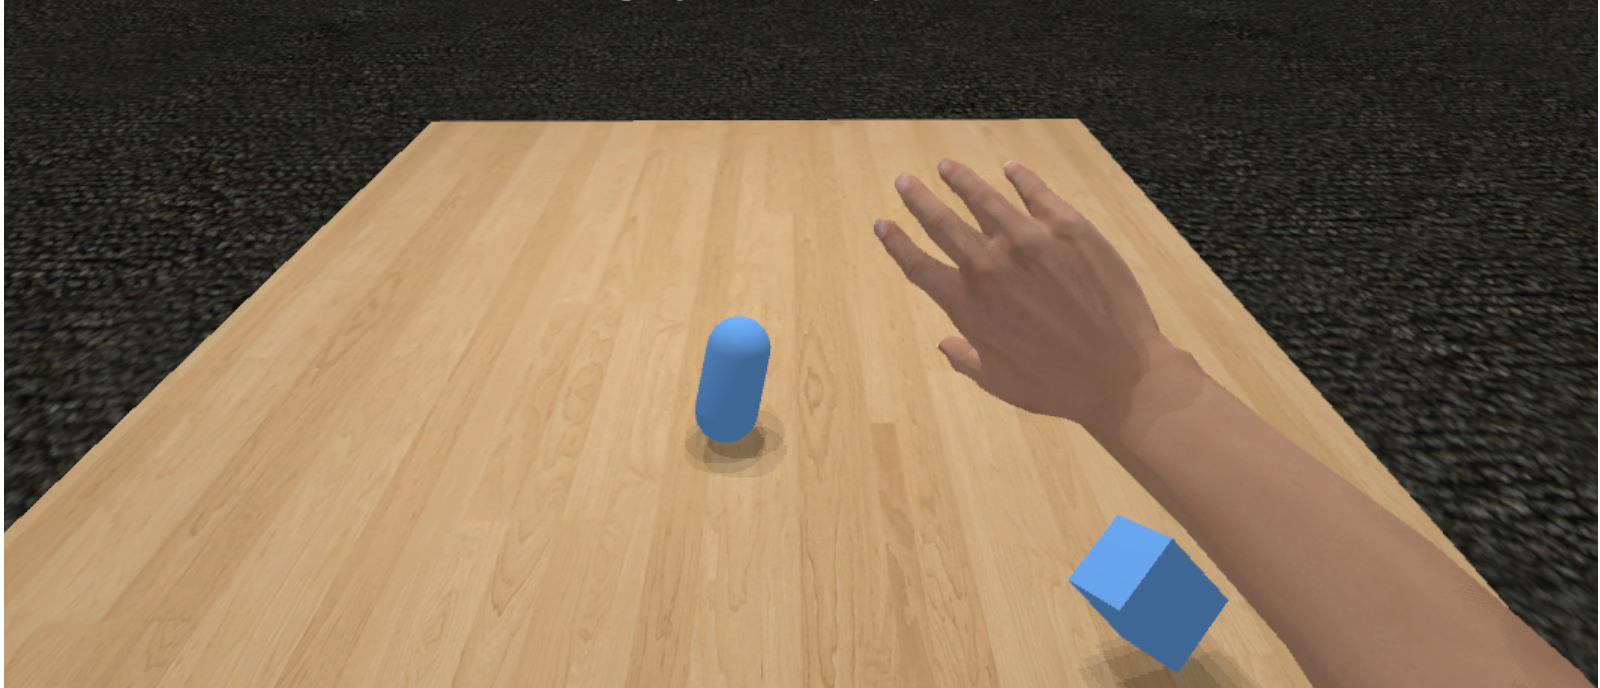
\includegraphics[width=\textwidth]{images/teaser.PNG}
    \caption{\label{fig:teaser} Visual Semantic Parsing process: The input of the algorithm is text and an RGB-D image. The result is a word to object alignment.}
}    

% Creates title of document and additional title page.
\maketitle 
 
\section*{Abstract}  
In their paper "What are you talking about? Text to image Coreference" ~\cite{urtasun2014} Uratsun et al. present their approach to improve 3D semantic parsing of images using sentential descriptions of scenes. The goal was to classify the scene, detect objects in the scene and most importantly to align noun/pronouns with those objects, which is the innovative idea of this project. In order to solve the word to object alignment task they used a Markov Random Field in which they jointly apply visual information parsed from the image and sentential information from natural descriptions of the scene. The results show that compared to a visual-only model the joint visual and textual model performs 14,4 \% better in scene classification and 6,4 \% better in object detection. The full model improves 2.3 \% over the unary-based alignment when evaluating nouns only. These are significant improvements compared to work that has been done in the field before (e.g. ~\cite{fidler2013} which is the closest to ~\cite{urtasun2014}) and the first of this kind when it comes to noun/pronoun to object alignment.
  
  
\section{Introduction}   
Object detection for us human beings is a very easy task. We also show a high flexibility even for detecting partly occluded objects or in general when it comes to detect objects under difficult circumstances. When it comes to scene detection we can usually tell in a split second what the current setting is about. Also when reading a description of an image it is quite easy for us to tell which words refer to certain objects in the image. In computer vision reliable object detection and scene classification has always been a challenge. In the paper ~\cite{urtasun2014} presented and reviewed here Urtasun et al. even go one step further and try to improve visual semantic parsing by also using sentential descriptions to make judgments about an image. Remarkable is the new approach to also align nouns and pronouns in the image with the according objects in the image. Compared to previous work in the field ~\cite{fidler2013} in which a similar approach was made this alignment process is the true innovation of the paper and can possibly lead to a major improvement in the way autonomous systems can interact with their environment. Therefore in this review the emphasis will be the methods used in the Text to Image Alignment Model of Urtasun et al.

\section{Text to Image Alignment Model} 
In their Text to Image Alignment Model Urtasun et al. use RGB-D images of an indoor scene as input as well as multi-sentence description of this scene. They let a Markov Random Field infer about the type of the scene, 3D detection as well as the alignment between nouns/pronouns and the objects in the scene.

\subsection{Input Data}
The images they use are simple RGB-D images from the challenging NYU/RGBD v2 dataset ~\cite{silberman2012} and there is nothing special to mention about them. However the sentential descriptions they use are special and have not been generated and used like this before. 
\paragraph{Data collection of sentential descriptions}
In order to get natural descriptions of the images they asked annotators (MTurkers) to describe the image as if they describe it to someone who doesn't see the image to give him/her a vivid impression of how the scene looks like. Multiple sentences per picture were possible which is new in the field and a more natural or realistic way in which text and images co-occur in the real world (e.g. captions of images, photo albums etc.). 
\paragraph{Coreference}
Using multiple sentences to describe a scene makes the alignment between nouns/pronouns with the objects in the image more challenging because of coreference. In linguistics coreference means that two or more words in a text can refer to the same person or thing. Therefore in the inference of the the Markov Random Model multiple mentions of the same object, its synonyms and pronouns referring to the same object have to be considered. In the next step all of the multiple mentions have to be aligned with the only correct instance of the object in the scene.

\subsection{Textual and Visual parsing} \label{Textual and Visual parsing}
In order to provide the Text to image alignment model with the relevant data, the raw input of the model (images and the according sentences) needs to be transformed into more specific data which then can be used as input nodes for the Markov Random Field. This is accomplished by Textual and visual parsing mechanisms.
\paragraph{Visual Parsing}
In order to parse textual descriptions the authors used Parts of Speech Tags (POS) which filter text for adjectives, nouns, verbs, pronouns etc. For this they used the Stanford POS Tagger for English Language ~\cite{toutanova2003}. They also applied type dependencies which are dependencies between individuals words such as word1 is subject and word2 is indirect object. Those type dependencies were found using the parsing methods of ~\cite{demarneffe2006} Nouns were detected with the POS and matched with object classes of interest (also their synonyms and plural forms). Classes of interest were generated by the visual parsing process. Attributes like 'brown' or 'on top of' were also extracted from the dependency information and used to analyze the spatial relations in the scene. In order to deal with pronouns and coreference the authors built clusters of coreferential mentions in the text. Such a cluster could be: 

\begin{labeling}{alligator}
\item [\textbf{noun1:}]    living room
\item [\textbf{noun2:}]    play room
\item [\textbf{pronoun1:}] it
\end{labeling}

All three words refer to the same instance of the scene. In this case the coreferential cluster contains all words referring to the the scene (classification) itself.

\begin{figure}[h!]
  \centering
  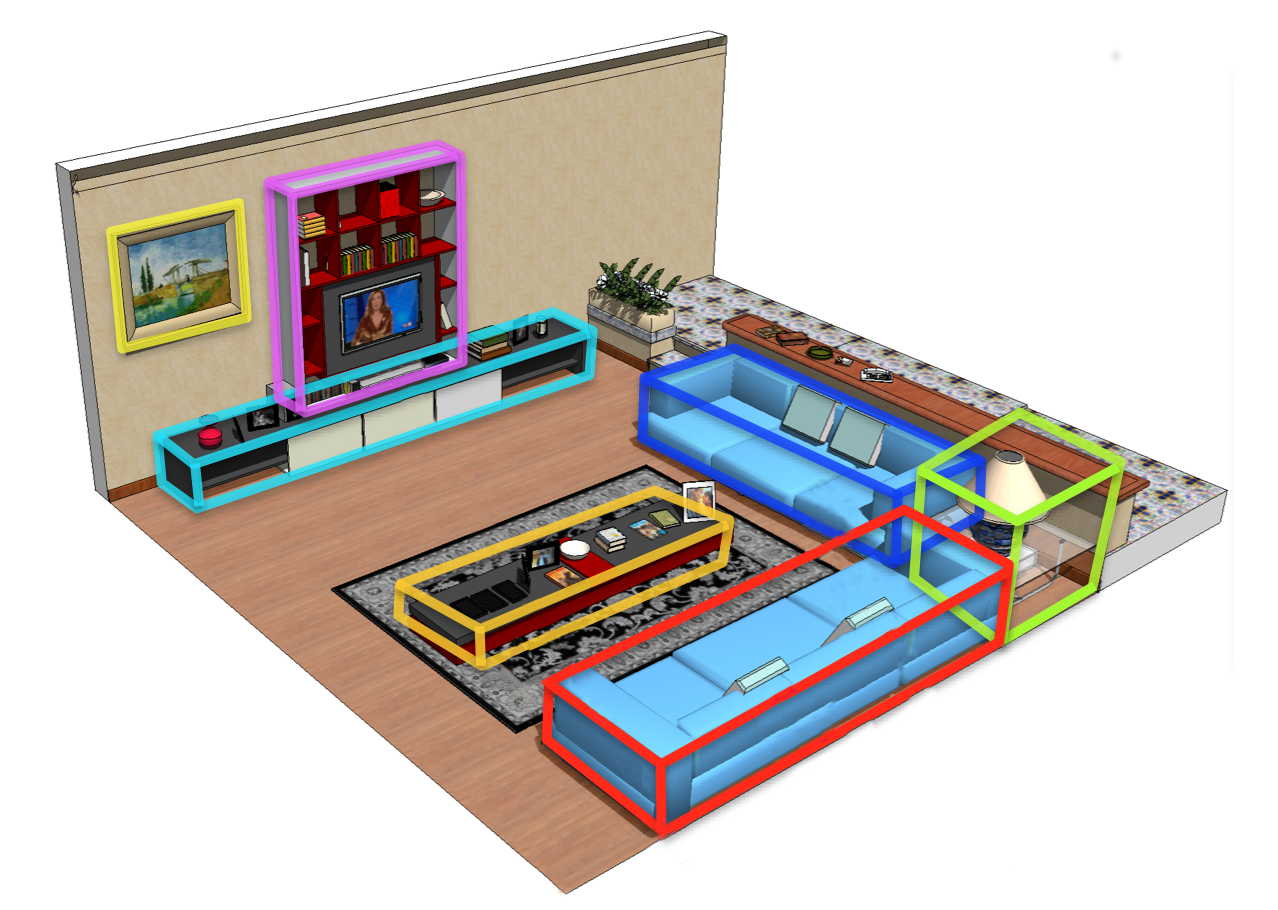
\includegraphics[width=.9\columnwidth]{images/scene_only_centered.png}
  \caption{\label{fig:3Dcuboids} The result of the parsing process from visual information to 3D cuboids.}
\end{figure}

\paragraph{Textual Parsing}
The parsing of visual information into 3D cuboids for each object in the scene was made in a three step process. First, regions of 3D objects in the scene were extracted via CPMC ~\cite{carreira2012}. Second, the regions were projected to 3D via RGB-D depth information. Finally a cuboid was fit around the detected 3D area of the object's region in the image (see Figure~\ref{fig:3Dcuboids}).

\subsection{Joint Visual and Textual Model} \label{Joint Visual and Textual Model}

In this section the Markov Random Field and its random variables that the authors used to jointly parse the visual and sentential input will be described. The type of scene was encoded in the random variable s. The semantic class of a candidate cuboid was encoded by the random variable $y_{(i)}$ (i is the i-th detected cuboid in the scene). Another indexing random variable $a_{(j)}$ was used for each noun/pronoun to select the cuboid that the noun refers to.

In Figure~\ref{fig:model} you can see a visual representation of the model which itself is very good. Unfortunately the authors did not sufficiently describe this figure in the text and they never really refer to what is seen in the figure. The only given explanation of the image can be found in the caption which says that black nodes and links represent visual information and blue nodes and links represent both textual and alignment information. 
Other than those links and nodes you can see two more nodes $a^{(1)}$ and $a^{(2)}$ representing two clusters of coreferential mentions as described in \ref{Textual and Visual parsing}. The cluster $a^{(1)}$ consists of the noun "sofas" and the pronoun "them". The cluster $a^{(2)}$ consists of the noun "table" only. Furthermore you can see two nodes $y^{(1)}$ and $y^{(2)}$ which represent cuboid instances which are the a result of the visual parsing process also described in \ref{Textual and Visual parsing}. 
The node s represents the random variable for the type of the scene, which is also indicated by the matrix on the right side. The matrix points with a green arrow to one of the black nodes $\phi_{so}$ which connects the node $y^{(2)}$ and the node s. This means that the detected sofa cuboid increases the likelihood of the random variable s in favor of the value "living room", which in this case is correct. The same applies for the node $\phi_{so}$ which connects $y^{(1)}$ and s. In this case $y^{(1)}$ simply represents another cuboid instance of another sofa in the scene.

\begin{figure*}[h!]
  \centering
  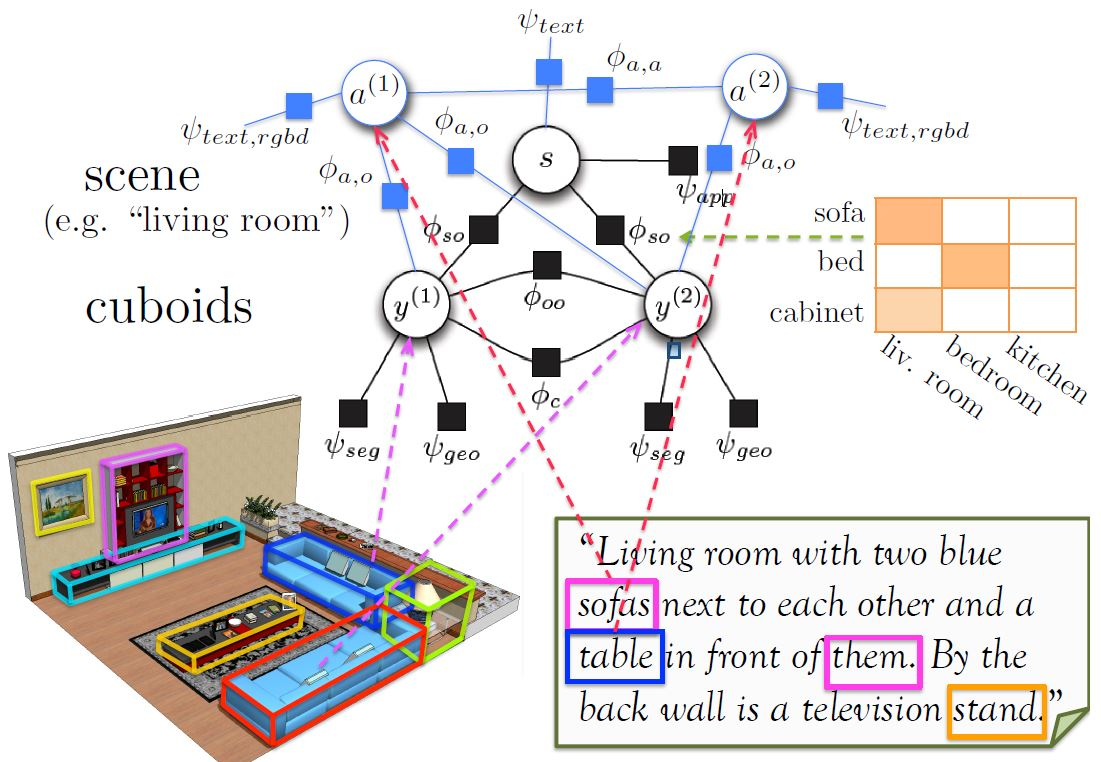
\includegraphics[width=1.5\columnwidth]{images/model.jpg}
  \caption{\label{fig:model}The joint visual and textual model. Black nodes and links represent visual information. Blue nodes and links represent both textual information and alignment information}
\end{figure*}

The notation of the labels of the square nodes differs from the author's description in the text so that it is hard to understand what they stand for. In the example of this figure the $\phi_{ao}$ nodes stand for alignment potentials between a cuboid ($y^{(1)}$ and $y^{(2)}$) and clusters of coreferential mentions of one object instance ($a^{(1)}$ and $a^{(2)}$) in the description. In other words the potentials $\phi_{ao}$ encode how likely it is that one cuboid instance refers to one cluster of coreferential mentions. In case $a^{(1)}$ which represents the cluster "sofas/them" we have two such $\phi_{ao}$ potentials linked from $a^{(1)}$ to each $y^{(1)}$ and $y^{(2)}$ because $y^{(1)}$ and $y^{(2)}$ actually represent the two "sofas" or "them". One can assume that those two potentials $\phi_{ao}$ are very high indicating a high likelihood that the two cuboids $y^{(1)}$ and $y^{(2)}$ can be aligned with the cluster "sofa/them". In case $a^{(2)}$ there is only one $\phi_{ao}$ alignment connection to $y^{(2)}$. Since $a^{(2)}$ represents the cluster which only consists of the word "table", but $y^{(2)}$ represents the cuboid of a sofa one can assume that this potential $\phi_{ao}$ must be very low, indicating that the cluster "table" and the sofa cuboid are very unlikely aligned.
For completeness the other potentials shown in the figure will be shortly explained in the following. The potential $\phi_{aa}$ must be the variety potential that they mention in their description. It is used for the plural mention of objects (here "sofas") in order to encourage the model to point to different cuboids via a pairwise potential. 

The nodes $\psi_{text, rgbd}$ must stand for joint visual and textual information that influences the random variables for the coreferential clusters (textual object instances). The node $\psi_{text}$ must stand for the text only input that influences the random variable s for the scene. The potentials $\phi_{oo)}$ and $\phi_{c}$ are not really clearly mentioned in the author's description, but it can be assumed that they are a spatial relation potential and a "same object class" potential. The potentials $\psi_{seg}$ and $\psi_{geo}$ represent segmentation and geometric features which characterize the cuboids. Those are not further described by the authors.

\newpage

\paragraph{Summary of the potentials and input nodes in Figure~\ref{fig:model}:}

\begin{labeling}{alligator}
\item [s:]    The type of the scene.
\item [$y_{(i)}$:]    The semantic class of a candidate cuboid.
\item [$a_{(j)}$:]    A selector for which cuboid each noun/pronoun refers to.
\item [$\phi_{so}$:]  Visual information of cuboid types that influence s. 
\item [$\phi_{ao}$:]    Likelihood that one cuboid instance refers to one cluster of coreferential mentions.
\item [$\phi_{aa}$:]   Varienty potential for plural mention of objects.
\item [$\phi_{oo}$:]    Spatial relation potential.
\item [$\phi_{c}$:]    Likelihood for same object class.
\item [$\psi_{text, rgbd}$:] Joint visual and textual information.
\item [$\psi_{text}$:]    Text only input that influences s.
\item [$\psi_{seg}$:] Segmentation information of cuboids.
\item [$\psi_{geo}$:] Geometric features of cuboids.
\end{labeling}

\subsection{Output of the Model}

In Figure~\ref{fig:results} heatmaps for the statistics of a mentioned object's location are shown. An interesting observation here was that people first describe closer and centered objects. The correlation between how early objects are mentioned in text and how important they are can be used in future work to further improve visual semantic parsing. In the paper presented here this observation was made, but not actually applied in the model.

\begin{figure}[h!]
  \centering
  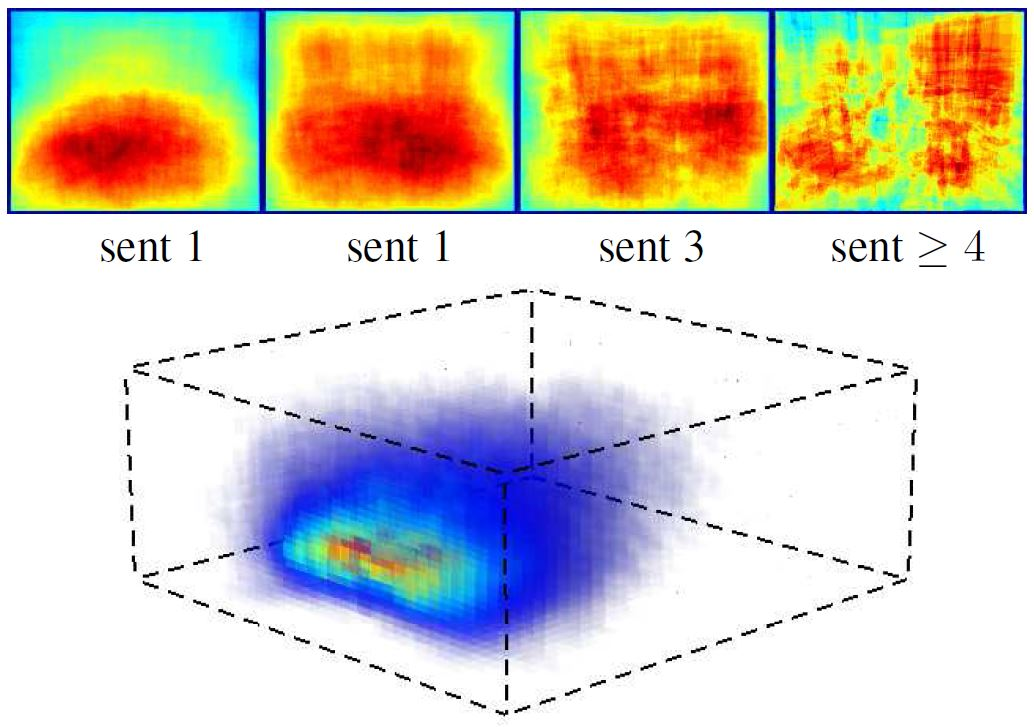
\includegraphics[width=.9\columnwidth]{images/results.jpg}
  \caption{\label{fig:results}Top: Location statistics of mentioned objects given which sentence mentions them. Bottom: Statistics of mentioned objects in 3D.}
\end{figure}

Figure~\ref{fig:alignment_example} shows an example output of the alignment between nouns/pronouns in text and objects/cuboids in the image. It shows how the model correctly aligns the word cabinet which is mentioned two times to the one cabinet instance in the image. Also the depth information of the cuboids is represented in different colors. Note that the parsing of visual information into 3D cuboids as described in Section \ref{Textual and Visual parsing} was not very accurate for the cabinet and the sink. The cabinet was actually only considered to be a rectangle instead of a cuboid. The location of the sink is spatially a little rotated. Nevertheless the alignment between words and the detected cuboids apparently works pretty well. Only the detection of correct cuboid boundaries for occluded or not very "cuboid-like" objects seemed to be not very reliable.

\begin{figure}[h!]
  \centering
  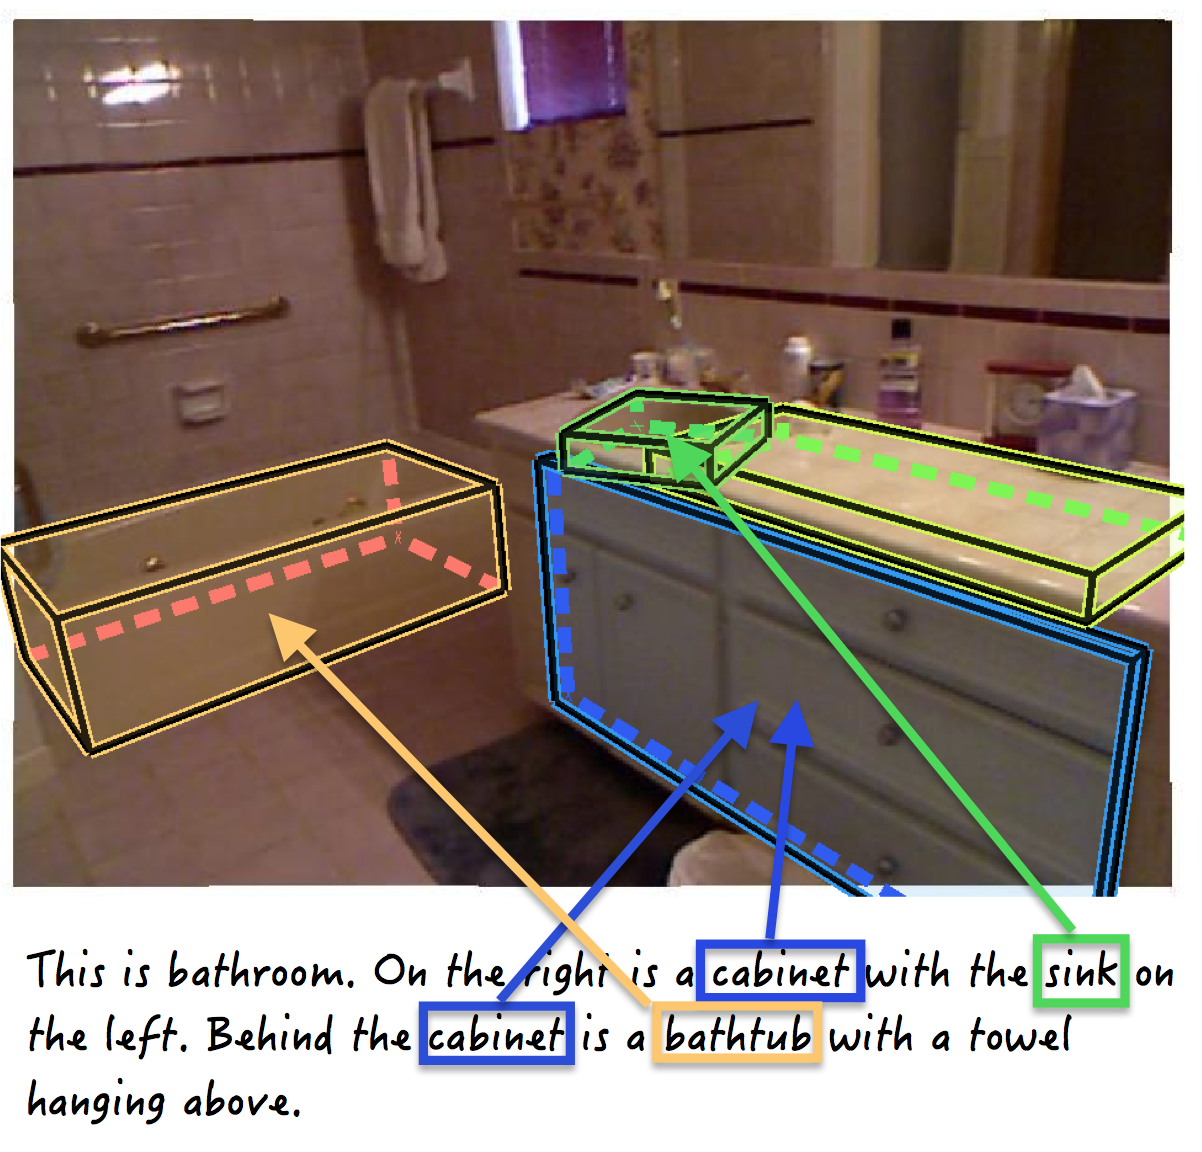
\includegraphics[width=.9\columnwidth]{images/result_actual_example.png}
  \caption{\label{fig:alignment_example} An actual example of how the resulting alignment of the model can look like.}
\end{figure}


\section{Personal Review}
Overall the paper is very nicely written and Urtasun et al. give a are able to give a good idea of their innovative work in Visual Semantic Parsing. However,  the relevant explanatory links of the figures in the text are missing sometimes. Therefore in this article an attempt was made to present a more detailed explanation of the central Figure \ref{fig:model} in ref{Section Joint Visual and Textual Model}. They mainly mention formulas of all the visual and textual potentials that they use, but little is said about how they work together. Therefore it is almost impossible to replicate their approach when only the information of the paper is given. On the website of Sanja Fidler who is one of the authors the dataset and the MathLab code that they used can be found ~\cite{fidler_online2014}. Also they present an interactive example page on which the alignment results can be tested by hovering the words in the text.

\section{Conclusion}
In their work Fidler and Urtasun showed that visual semantic parsing can be significantly improved by using textual descriptions of images in a joint visual and textual model. The improvement over the visual only model is 14,4 \% for scene classification, 6,4 \% for object detection and the full model improves 2,3 \% over the unary based alignment when evaluating nouns only. Especially the high accuracy in text to object alignment is remarkable and could be used in the future to train autonomous systems to apply this information in real time tasks.

\bibliographystyle{alpha}
\bibliography{bibliography}

\end{document}

